\documentclass{article}
% Chinese
% \documentclass[UTF8, nofonts, mathptmx, 12pt, onecolumn]{article}
% \usepackage{xeCJK}
% \setCJKmainfont{SimSun}
\usepackage{amsmath}
\usepackage{amsfonts}
\usepackage{amssymb}
\usepackage{wasysym}
% \usepackage{ctex}
\usepackage{graphicx}
\usepackage{float}
\usepackage{geometry}
\geometry{a4paper,scale=0.8}
\usepackage{caption}
\usepackage{subcaption}
% \newcommand{\oiint}{\mathop{{\int\!\!\!\!\!\int}\mkern-21mu \bigcirc} {}}
\newcommand*{\dif}{\mathop{}\!\mathrm{d}}
\newcommand*{\md}{\mathop{}\!\mathrm{d}}
\newcommand*{\me}{\mathrm{e}}

% \usepackage{parskip}
% \setlength{\parindent}{0cm}

\usepackage{bm}
\let\Oldmathbf\mathbf
\renewcommand{\mathbf}[1]{\boldsymbol{\Oldmathbf{#1}}}
\let\eqnarray\align

\author{Xiping Hu}
\usepackage{authblk}
\author{Xiping Hu}
\affil{https://hxp.plus/}
\title{Homework for Chapter 4}

\begin{document}
\maketitle

\begin{figure}[H]
  \centering
  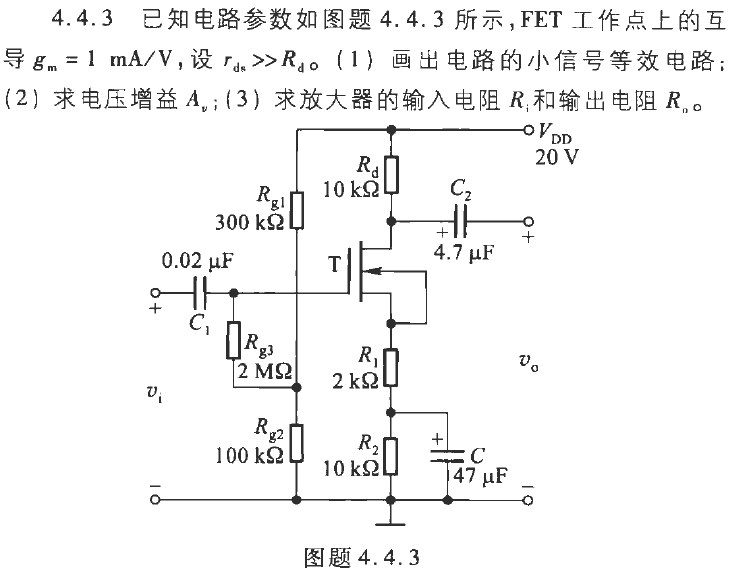
\includegraphics[width=\linewidth]{figures/Problem443}
  \label{fig:}
\end{figure}

\paragraph{Problem 1}

The circuit for small signal is shown below

\begin{figure}[H]
  \centering
  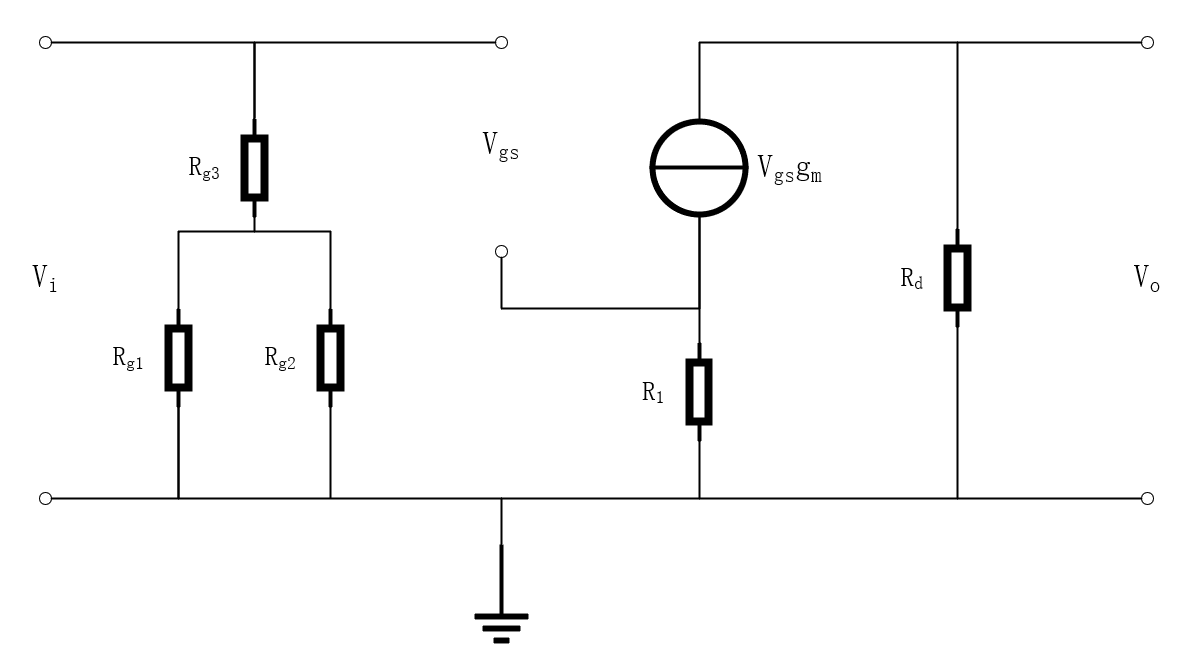
\includegraphics[width=\linewidth]{figures/Problem4431}
  \label{fig:}
\end{figure}

\paragraph{Problem 2}

\begin{equation*}
  \begin{aligned}
    A_v = \dfrac{V_o}{V_i} = \dfrac{- g_m V_{gs} R_d}{V_{gs} + g_m V_{gs} R_1} = - 3.3 
  \end{aligned}
\end{equation*}

\paragraph{Problem 3}

\begin{equation*}
  \begin{aligned}
    R_i = R_{g3} + \dfrac{R_{g1} R_{g_2}}{R_{g1} + R_{g2}} =  2075 \  \mathrm{k \Omega}
  \end{aligned}
\end{equation*}



\end{document}